\documentclass[12pt]{sprawozdanie}

\class{Informatyka II}
\title{Układ ze sprężyną o nieliniowej charakterystyce}
\author{\textbf{Jan Adamski} 123456\\\textbf{Adam Jański} 654321}
\instructor{Jakiś Ktoś}
\deadline{01.06.2019 r.}

\begin{document}
\maketitle
\hypertarget{opis-problemu}{%
\section{Opis problemu}\label{opis-problemu}}

\begin{center}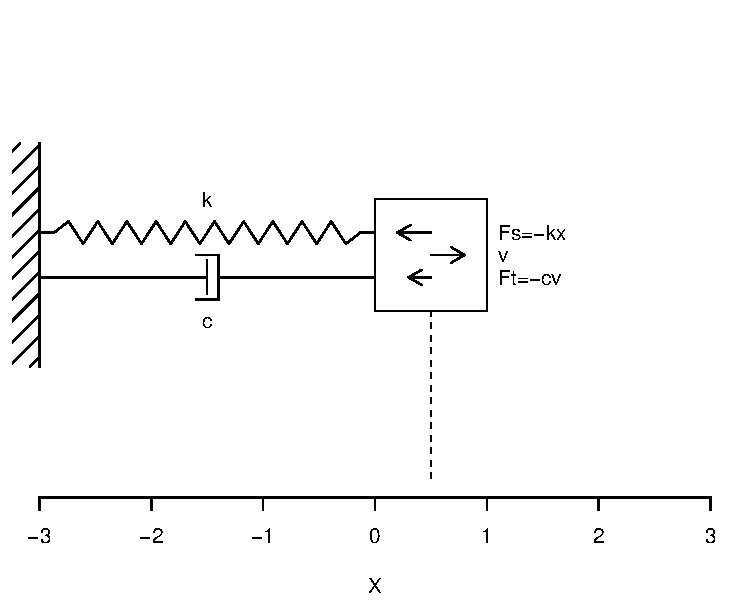
\includegraphics{info2_files/figure-latex/scheme-1} \end{center}

Charakterystyka nieliniowa sprężyny: \(k=k_1(1+k_2x^2)\)

\hypertarget{rownania-ruchu}{%
\section{Równania ruchu}\label{rownania-ruchu}}

Siła wywierana na masę przez sprężynę: \[F_s = -kx = -k_1(1+k_2x^2)x\]
Siła wywierana na masę przez tłumik: \[F_t = -c\dot x\] Równanie ruchu:
\[m\ddot x = F_s + F_t = -k_1(1+k_2x^2)x-c\dot x\] Równanie to można
przekształcić na układ równań pierwszego rzędu:
\begin{equation}\label{uklad}\begin{cases}
\dot x &= y\\
\dot y &= \frac{1}{m}\left(-k_1(1+k_2x^2)x - cy\right)
\end{cases}\end{equation}

Energia kinetyczna: \[E_k = \frac{m\dot x^2}{2}\] Energia potencjalna
sprężyny:
\[E_p = \int k_1(1+k_2x^2)x\cdot dx = \int \left(k_1x+k_1k_2x^3\right)dx = \frac{k_1x^2}{2}+\frac{k_1k_2x^4}{4}\]
Całkowita energia mechaniczna:
\[E = \frac{m\dot x^2}{2} + \frac{k_1x^2}{2}+\frac{k_1k_2x^4}{4}\]

\textbf{Uwaga:} bez straty ogólności, w dalszej części pracy będziemy
przyjmować \(m=1\).

\hypertarget{metoda-obliczeniowa}{%
\section{Metoda Obliczeniowa}\label{metoda-obliczeniowa}}

Układ równań został scałkowany przy pomocy metody Runge-Kutta 4-tego
rzędu. Czas całkowania: \(10s\). Krok całkowania: \(\frac{10s}{1500}\).

\hypertarget{wyniki}{%
\section{Wyniki}\label{wyniki}}

Przeprowadzono symulację dla czterech przypadków: Liniowej i nieliniowej
charakterystyki sprężyny, a także z i bez tłumienia.

\hypertarget{przypadek-liniowej-sprezyny-k_110}{%
\subsection{\texorpdfstring{Przypadek liniowej sprężyny
(\(k_1=10\))}{Przypadek liniowej sprężyny (k\_1=10)}}\label{przypadek-liniowej-sprezyny-k_110}}

Liniowa sprężyna charakteryzuje się liniową zależnością pomiędzy
wychyleniem a siłą:

\begin{center}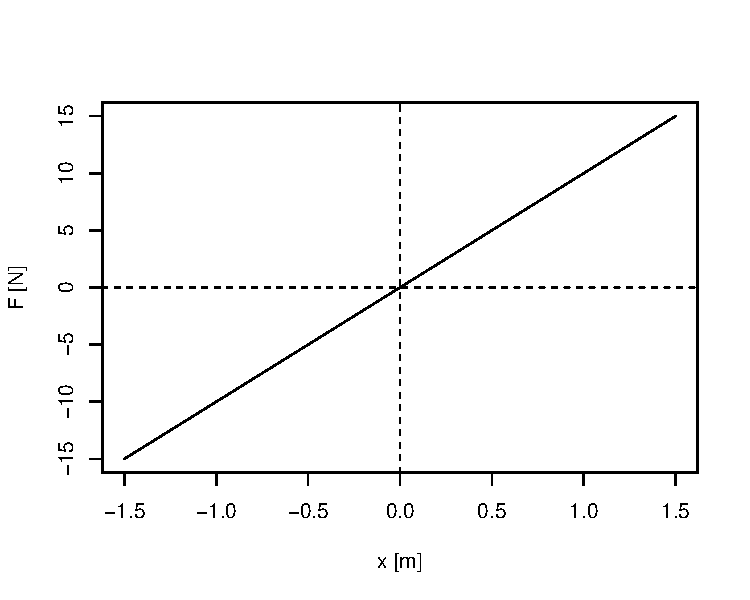
\includegraphics{info2_files/figure-latex/linear-characteristic-1} \end{center}

Rozwiązanie numeryczne tego układu jest zgodne z oczekiwanym
sinusoidalnym kształtem:

\begin{center}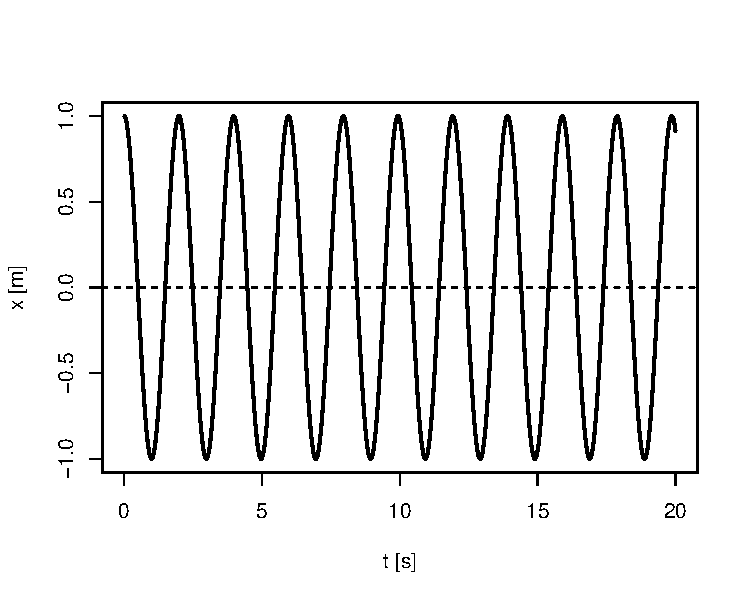
\includegraphics{info2_files/figure-latex/linear-solution-1} \end{center}

Dla tak prostego układu \(m\ddot x + k_1x = 0\), możemy wyznaczyć
rozwiązanie analityczne przez podstawienie \(x=e^{rt}\). Otrzymane
rozwiązanie ogólne (po usunięciu części urojonej) ma postać:
\[x(t) = A \cos{\sqrt{\frac{k_1}{m}}t} + B \sin{\sqrt{\frac{k_1}{m}}t}\]
Dla warunków początkowych \(x(0)=1\land \dot x(0)=1\) mamy:
\[x(t) = \cos{\sqrt{\frac{k_1}{m}}t}\]

Wizualnie rozwiązanie numeryczne pokryłoby się z analitycznym, możemy
jednak zwizualizować błąd względny
(\(\left|\frac{x_n-x_a}{x_a}\right|\)) w skali logarytmicznej:

\begin{center}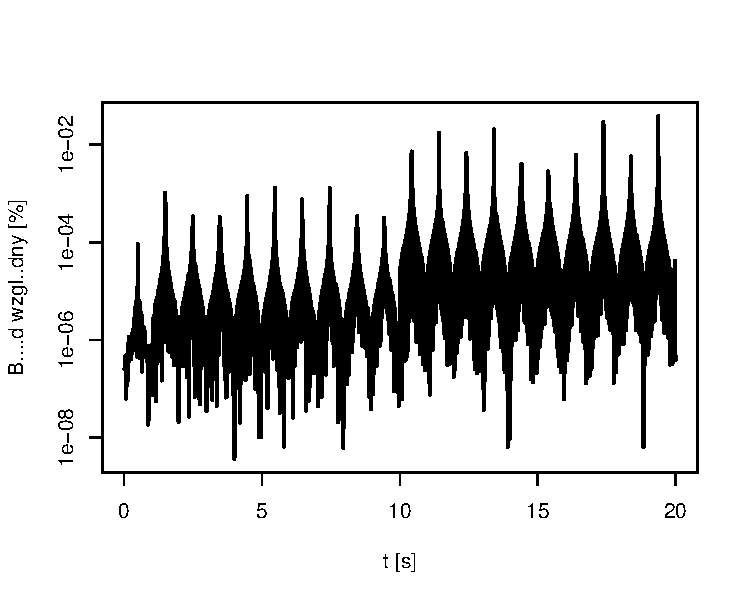
\includegraphics{info2_files/figure-latex/linear-error-1} \end{center}

W przestrzeni fazowej (\(x-v\)) rozwiązanie jest zamkniętą elipsą. Nie
ma tu sensu mówienie o jej proporcjach, ponieważ obie osie mają różne
skale.

\begin{center}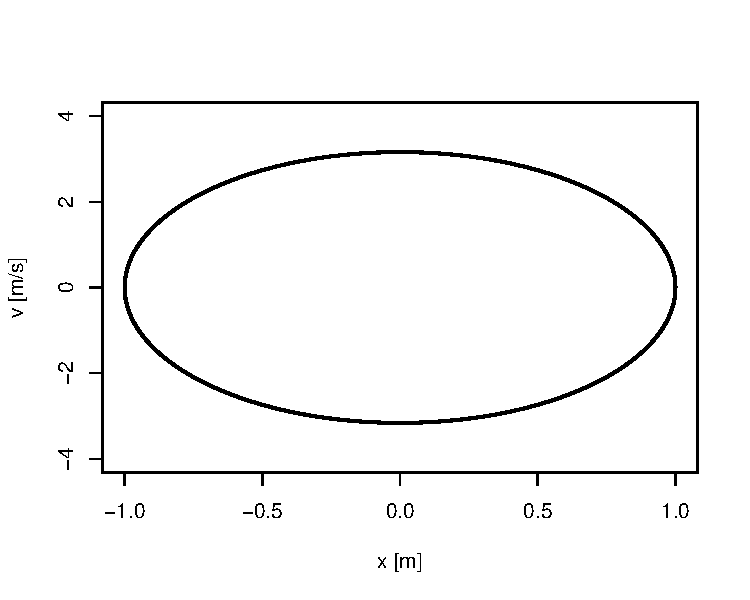
\includegraphics{info2_files/figure-latex/linear-phase-space-1} \end{center}

Zamknięta ścieżka w przestrzeni fazowej sugeruje, że układ nie traci
energii.

\hypertarget{przypadek-nieliniowej-sprezyny-k_15quad-k_23}{%
\subsection{\texorpdfstring{Przypadek nieliniowej sprężyny
(\(k_1=5\quad k_2=3\))}{Przypadek nieliniowej sprężyny (k\_1=5\textbackslash{}quad k\_2=3)}}\label{przypadek-nieliniowej-sprezyny-k_15quad-k_23}}

Zależność siły od wychylenia dla omawianej nieliniowej sprężyny:

\begin{center}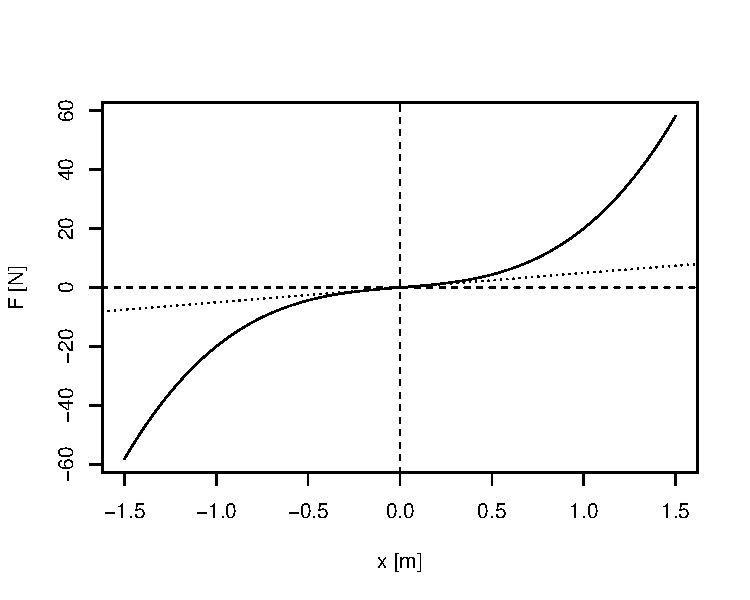
\includegraphics{info2_files/figure-latex/nonlinear-characteristic-1} \end{center}

Rozwiązanie numeryczne dla nieliniowej sprężyny ma ``ostrzej''
zakończone maxima i minima. Jest to związane z wyższą siłą siłą przy
dużych wychyleniach niż w przypadku liniowej sprężyny.

\begin{center}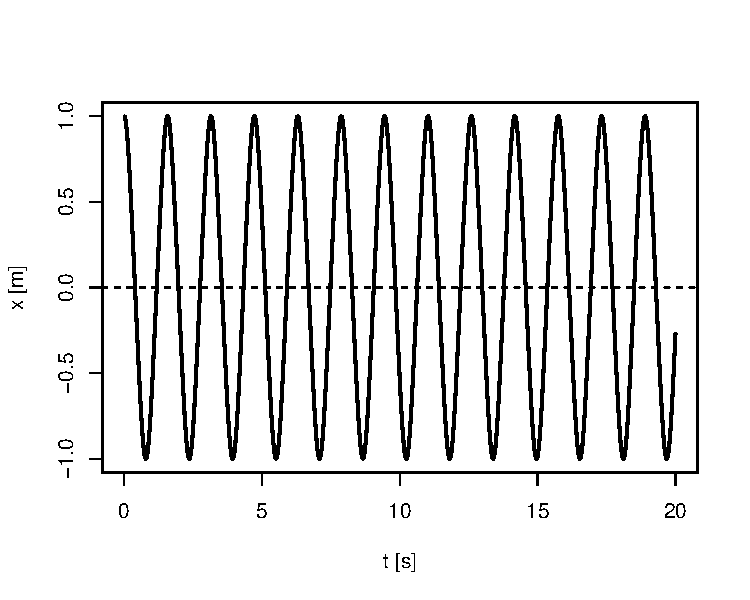
\includegraphics{info2_files/figure-latex/nonlinear-solution-1} \end{center}

W przestrzeni fazowej, trajektoria nadal jest zamkniętą pętlą, lecz nie
jest już elipsą:

\begin{center}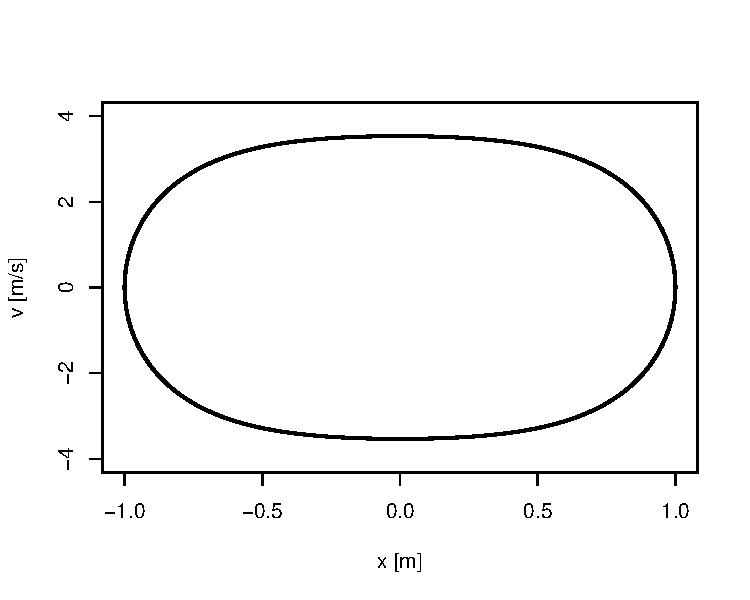
\includegraphics{info2_files/figure-latex/nonlinear-phase-1} \end{center}

\hypertarget{przypadek-liniowej-sprezyny-z-tumikiem-k_110quad-c0.3}{%
\subsection{\texorpdfstring{Przypadek liniowej sprężyny z tłumikiem
(\(k_1=10\quad c=0.3\))}{Przypadek liniowej sprężyny z tłumikiem (k\_1=10\textbackslash{}quad c=0.3)}}\label{przypadek-liniowej-sprezyny-z-tumikiem-k_110quad-c0.3}}

Rozwiązanie numeryczne dla liniowej sprężyny z tłumikiem, ma wykładniczy
spadek. W związku z tym, że częstotliwość drgania układu liniowego nie
zależy od wychylenia, odstępy pomiędzy momentami przejścia przez zero są
ciągle stałe.

\begin{center}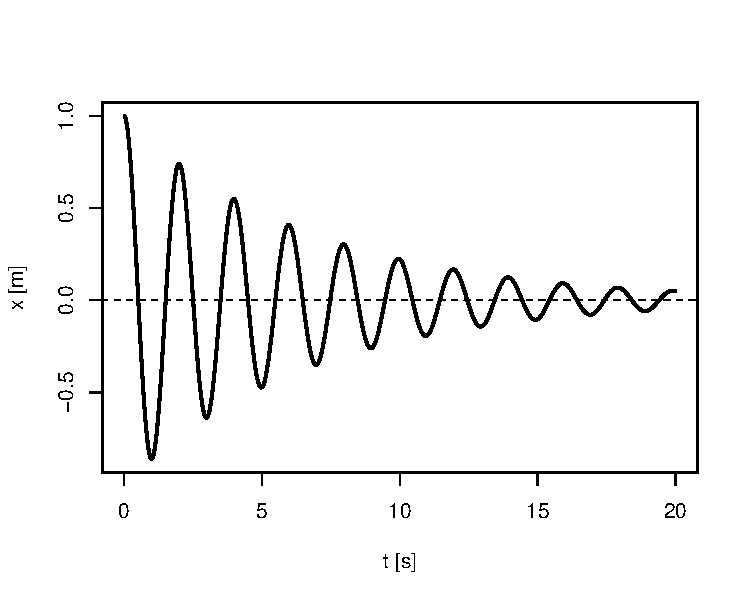
\includegraphics{info2_files/figure-latex/linear-dump-solution-1} \end{center}

W przestrzeni fazowej, trajektoria nie jest już zamknięta i schodzi
spiralnie do zera:

\begin{center}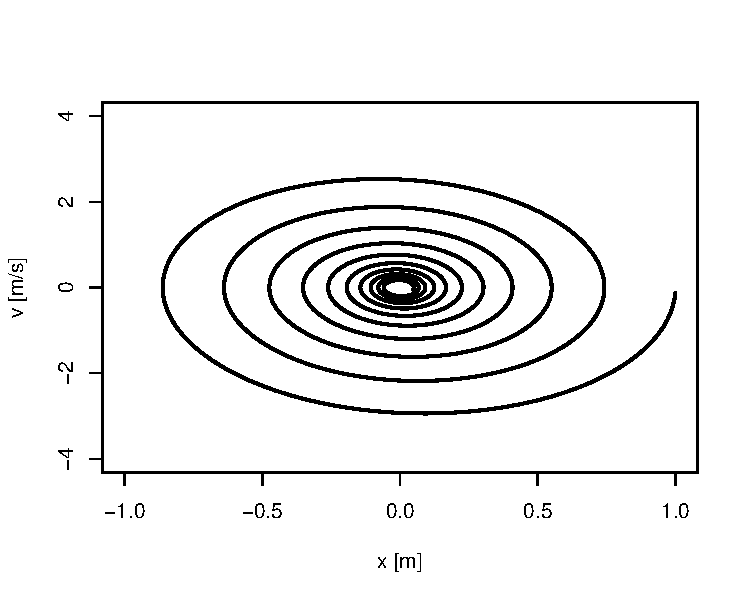
\includegraphics{info2_files/figure-latex/linear-dump-phase-1} \end{center}

Tłumik wprowadza element niezachowawczy do układu. Powoduje to spadek
energii. Łatwo ten efekt zobaczyć wymnażając oryginalny układ przez
\(\dot x\): \[\dot xm\ddot x + \dot xc\dot x + \dot xk_1x=0\] Po
przekształceniu mamy:
\[\frac{d}{dt}\left(\frac{m\dot x^2}{2}+\frac{k_1 x^2}{2}\right)=-c\dot x^2\]
Na wykresie całkowitej energii widać wyraźnie spadek energii, który
następuje w momentach wysokiej prędkości.

\begin{center}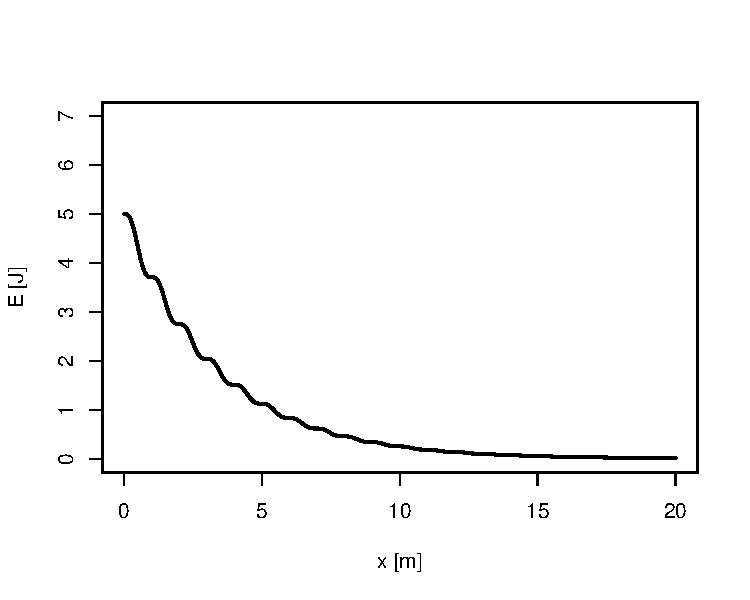
\includegraphics{info2_files/figure-latex/linear-dump-energy-1} \end{center}

\hypertarget{przypadek-nieliniowej-sprezyny-z-tumikiem-k_15quad-k_23quad-c0.3}{%
\subsection{\texorpdfstring{Przypadek nieliniowej sprężyny z tłumikiem
(\(k_1=5\quad k_2=3\quad c=0.3\))}{Przypadek nieliniowej sprężyny z tłumikiem (k\_1=5\textbackslash{}quad k\_2=3\textbackslash{}quad c=0.3)}}\label{przypadek-nieliniowej-sprezyny-z-tumikiem-k_15quad-k_23quad-c0.3}}

Rozwiązanie numeryczne dla nie-liniowej sprężyny z tłumikiem, ma także
wykładniczy spadek. Dla nieliniowej sprężyny częstotliwość zmienia się
wraz z maksymalnym wychyleniem. Dlatego odstępy pomiędzy przejściami
przez zero będą się wydłużać.

\begin{center}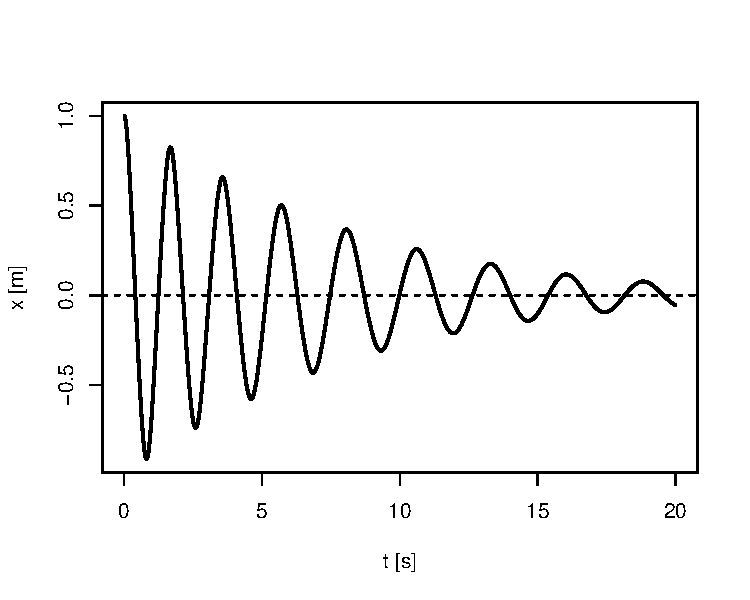
\includegraphics{info2_files/figure-latex/nonlinear-dump-solution-1} \end{center}

W przestrzeni fazowej, trajektoria jest nieeliptyczną spiralą. Dodatkowo
można zauważyć że gdy wychylenie się zmniejsza, trajektoria robi się
coraz bardziej eliptyczna:

\begin{center}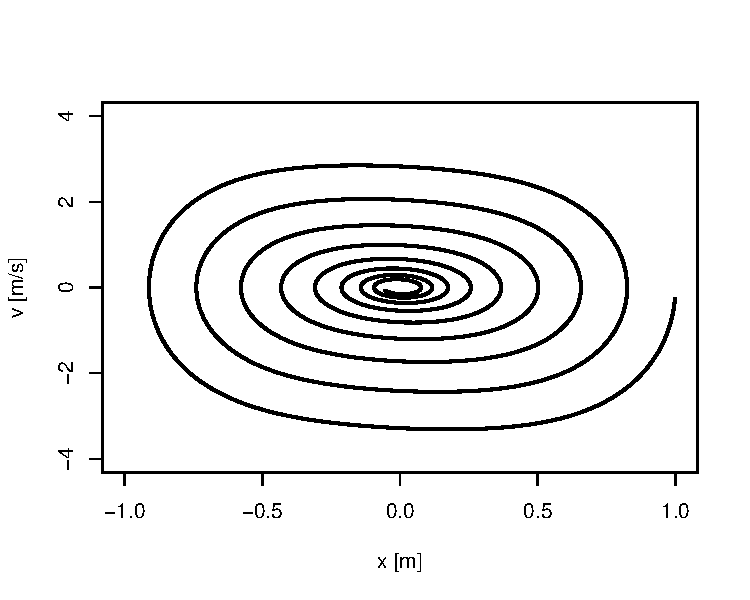
\includegraphics{info2_files/figure-latex/nonlinear-dump-phase-1} \end{center}

Tak jak w poprzednim przypadku, energia spada w czasie:

\begin{center}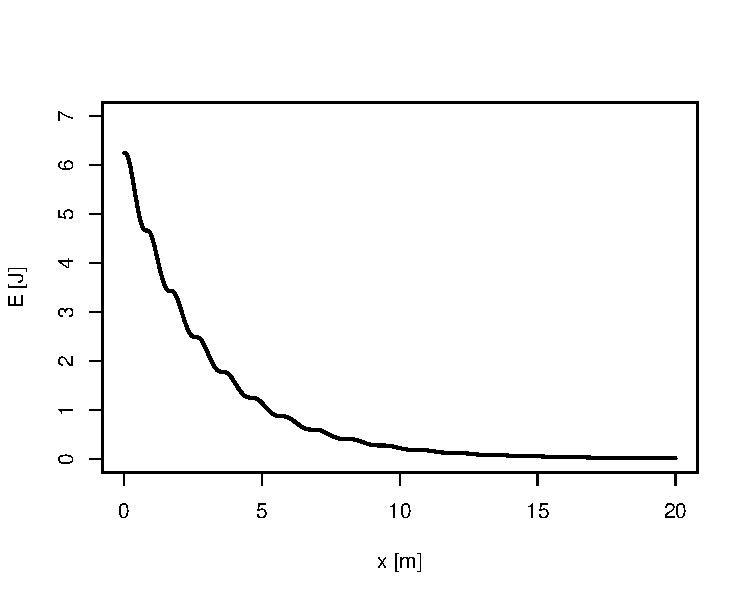
\includegraphics{info2_files/figure-latex/nonlinear-dump-energy-1} \end{center}

\hypertarget{omowienie-wynikow}{%
\section{Omówienie wyników}\label{omowienie-wynikow}}
\end{document}
